\chapter{Implementation and software examples}
\label{sec:implementation}

\begin{table}[t]
  \centering
  \caption{Dimensions for the settings considered in this section}
  \label{tab:sizes}
\resizebox{\textwidth}{!}{
\begin{tabular}{lll}\toprule
  Setting & Context dimension $|\gX|$ & Solution dimension $|\gY|$ \\ \midrule
  VAE on MNIST (\ref{sec:impl:vaes}) & $784$ {\color{gray} (=$28\cdot 28$, MNIST digits)} & $20$ {\color{gray}(parameterizing a 10D Gaussian)} \\
  Model-free control (\ref{sec:impl:model-free}) & $45$ {\color{gray}(humanoid states)} & $17$ {\color{gray} (action dimension)} \\
  Model-based control (\ref{sec:impl:model-based}) & $45$ {\color{gray}(humanoid states)} & $51$ {\color{gray} (=$17\cdot 3$, short action sequence)} \\
  Sphere (\ref{sec:impl:sphere}) & $16$ {\color{gray}($c$-convex function parameterizations)} & $3$ {\color{gray} (sphere)} \\ \bottomrule
\end{tabular}}
\end{table}

Turning now to the implementation details, this section
looks at how to develop and analyze amortization software.
The standard and easiest approach in most settings is to use
automatic differentiation software such as
\citet{maclaurin2015autograd,al2016theano,abadi2016tensorflow,bezanson2017julia,agrawal2019tensorflow,paszke2019pytorch,bradbury2020jax}
to parameterize and learn the amortization model.
There are many open source implementations and re-implementations
of the methods in \cref{sec:apps} that provide a concrete
starting point to start building on them.
This section looks closer at three specific implementations:
\cref{sec:impl:eval} evaluates the amortization components
behind existing implementations of variational autoencoders
\cref{sec:apps:avi} and control \cref{sec:apps:ctrl} and
\cref{sec:impl:sphere} implements and trains an amortization model
to optimize functions defined on a sphere.
\Cref{tab:sizes} summarizes the concrete dimensions of the amortization
problems considered here and \cref{sec:impl:software}
concludes with other useful software references.
The source code behind this section is available at
\url{https://github.com/facebookresearch/amortized-optimization-tutorial}.

\section{Amortization in the wild: a deeper look}
\label{sec:impl:eval}

This section shows code examples of how existing implementations
using amortized optimization define and optimize their models
for variational autoencoders (\cref{sec:impl:vaes})
and control and policy learning (\cref{sec:impl:model-free,sec:impl:model-based}).
The amortization component in these systems is often a part
of a larger system to achieve a larger task:
VAEs also reconstruct the source data
after amortizing the ELBO computation in \cref{eq:vae-full}
and policy learning methods also estimate the
$Q$-value function in \cref{sec:Q-learning}.
This section scopes to the amortization components to show
how they are implemented.
I have also added evaluation code to the pre-trained amortization models
from existing repositories and show that the amortized approximation
often obtains a solution up to \textbf{25000 times} faster than
solving the optimization problems from scratch on an
NVIDIA Quadro GP100 GPU.

\subsection{The variational autoencoder (VAE)}
\label{sec:impl:vaes}

This section looks at the code behind
standard VAE \citep{kingma2013auto} that follows the
amortized optimization setup described in \cref{sec:apps:vae}.
While there are many implementations for training and
reproducing a VAE, this section will use the implementation at
\url{https://github.com/YannDubs/disentangling-vae},
which builds on the code behind
\citet{dupont2018learning} at
\url{https://github.com/Schlumberger/joint-vae}.
While the repository is focused on disentangled representations
and extensions of the original VAE formulation, this
section only highlights the parts corresponding to the
original VAE formulation.
The code uses standard PyTorch in a minimal way that
allow us to easily look at the amortization components.

\textbf{Training the VAE.}
\Cref{lst:vae} paraphrases the relevant snippets of code to
implement the main amortization problem in \cref{eq:vae-amor}
for image data where the likelihood is given by a Bernoulli.
\Cref{lst:vae.encoder} defines an encoder $\hat \lambda_\theta$,
to predicts a solution to the ELBO implemented in \cref{lst:vae.elbo},
which is optimized in a loop over the training data (images)
in \cref{lst:vae.loop}.
The \path{README} in the repository contains instructions
for running the training from scratch.
The repository contains the binary of a model trained
on the MNIST dataset \citep{lecun1998mnist}, which
the next portion evaluates.

\begin{figure}[t]
  \centering
  \vspace{-4mm}
  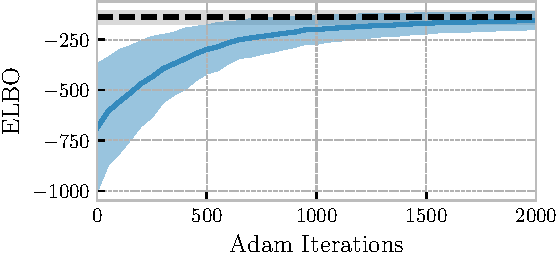
\includegraphics[width=0.49\textwidth]{fig/vae-iter.pdf}
  \hfill
  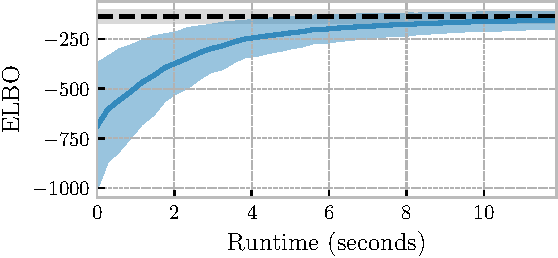
\includegraphics[width=0.49\textwidth]{fig/vae-time.pdf} \\
  \cblock{0}{0}{0} Amortized encoder $\hat\lambda_\theta(x)$ --- runtime: 0.4ms
  \caption{
    Runtime comparison between Adam and an amortized encoder $\hat\lambda_\theta$
    to solve \cref{eq:elbo-opt} for a VAE on MNIST.
    This uses a batch of 1024 samples and was
    run on an unloaded NVIDIA Quadro GP100 GPU.
    The values are normalized so that $\lambda(x)=0$ takes a value of -1 and
    the optimal $\lambda^\star$ takes a value of 0.
    The amortized policy is approximately
    \textbf{25000} times faster than solving the
    problem from scratch.
  }
  \label{fig:vae-performance}
\end{figure}

\begin{figure}
  \centering
\begin{subfigure}[b]{\textwidth}
\begin{lstlisting}
class Encoder(nn.Module): # From disvae.models.encoders
    def forward(self, x): # x is the amortization context: the original data
        mu_logvar = self.convnet(x)
        mu, logvar = mu_logvar.view(-1, self.latent_dim, 2).unbind(-1) # Split
        return (mu, logvar) # = latent_dist or \lambda
\end{lstlisting}
\caption{Forward definition for the encoder $\hat \lambda_\theta(x)$.
  \path{self.convnet} uses the architecture
  from \citet{burgess2018understanding}.}
\label{lst:vae.encoder}
\end{subfigure}
\begin{subfigure}[b]{\textwidth}
\begin{lstlisting}
# From disvae.models.losses.BetaHLoss with a Bernoulli likelihood
def estimate_elbo(data, latent_dist):
    mean, logvar = latent_dist

    reconstructed_batch = sample_and_decode(latent_dist)
    log_likelihood = -F.binary_cross_entropy(
        reconstructed_batch, x, reduce=False).sum(dim=[1,2,3])

    # Closed-form distance to the prior
    latent_kl = 0.5 * (-1 - logvar + mean.pow(2) + logvar.exp())
    kl_to_prior = latent_kl.sum(dim=[-1])

    loss = log_likelihood - kl_to_prior
    return loss.mean()
\end{lstlisting}
\caption{Definition of the $\ELBO$ in \cref{eq:elbo}}
\label{lst:vae.elbo}
\end{subfigure}

\begin{subfigure}[b]{\textwidth}
\begin{lstlisting}
model = Encoder()
for batch in iter(data_loader):
    latent_dist = model(batch)
    loss = -estimate_elbo(batch, latent_dist)
    self.optimizer.zero_grad()
    loss.backward()
    self.optimizer.step()
\end{lstlisting}
\caption{Main VAE training loop for the encoder}
\label{lst:vae.loop}
\end{subfigure}

\caption{Paraphrased PyTorch code examples of the key
  amortization components of a VAE from
  \url{https://github.com/YannDubs/disentangling-vae}.}
\label{lst:vae}
\end{figure}

\textbf{Evaluating the VAE.}
This section looks at how well the amortized encoder
$\hat\lambda$ approximates the optimal
encoder $\lambda^\star$ given by explicitly solving
\cref{eq:elbo-opt}, which is
referred to the \emph{amortization gap} \citep{cremer2018inference}.
\cref{eq:elbo-opt} can be solved with a gradient-based optimizer
such as SGD or Adam \citep{kingma2014adam}.
\Cref{lst:evaluation} shows the key parts of the PyTorch code
for making this comparison, which can be run on the pre-trained
MNIST VAE with
\path{code/evaluate_amortization_speed_function_vae.py}.

\Cref{fig:vae-performance} shows that the amortized prediction from
the VAE's encoder predicts the solution to the ELBO \textbf{25000}
times faster (!) than running 2k iterations of Adam on
a batch of 1024 samples.
This is significant as \emph{every training iteration} of
the VAE requires solving \cref{eq:elbo-opt}, and a large model
may need millions of training iterations to converge.
Amortizing the solution makes the difference between the training
code running in a few hours instead of a few months if
the problem was solved from scratch to the same level of optimality.
Knowing only the ELBO values is not sufficient to gauge
the quality of approximate variational distributions.
To help understand the quality of the approximate solutions,
\cref{fig:vae-samples} plots out the decoded samples
alongside the original data.

\begin{figure}[t]
  \centering
  \resizebox{\textwidth}{!}{
  \hspace*{-4mm}
  \begin{tikzpicture}
    \node[align=left,anchor=north west] {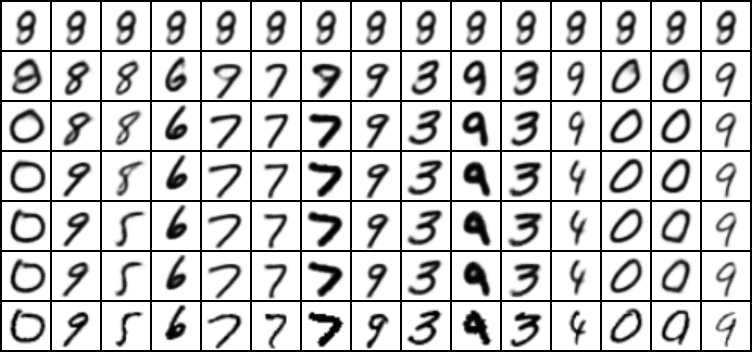
\includegraphics[width=430pt]{fig/vae-samples.png}};
    \node[align=right,anchor=east] at (2mm,-6mm) (0) {0};
    \node[align=right,below=10.3mm of 0.east,anchor=east] (250) {${\rm Adam}_{250}$};
    \node[align=right,below=10.3mm of 250.east,anchor=east] (500) {${\rm Adam}_{500}$};
    \node[align=right,below=10.3mm of 500.east,anchor=east] (1000) {${\rm Adam}_{1000}$};
    \node[align=right,below=10.3mm of 1000.east,anchor=east] (2000) {${\rm Adam}_{2000}$};
    \node[align=right,below=10.3mm of 2000.east,anchor=east] (amor) {$\hat\lambda_\theta(x)$};
    \node[align=right,below=9.5mm of amor.east,anchor=east] (data) {Data};
  \end{tikzpicture}}
\caption{Decoded reconstructions of the variational distribution optimizing for the ELBO.
  ${\rm Adam}_n$ corresponds to the distribution from running Adam for $n$
  iterations, $\hat \lambda_\theta$ is the amortized approximation,
  and the ground-truth data, \ie the context, is shown in the bottom row.
}

  \label{fig:vae-samples}
\end{figure}

\begin{figure}[t]
\begin{lstlisting}
# amortization_model: maps contexts to a solution
# amortization_objective: maps an iterate and contexts to the objective

adam_lr, num_iterations = ...
contexts = sample_contexts()

# Predict the solutions with the amortization model
predicted_solutions = amortization_model(contexts)
amortized_objectives = amortization_objective(
    predicted_solutions, contexts
)

# Use Adam (or another torch optimizer) to solve for the solutions
iterates = torch.nn.Parameter(torch.zeros_like(predicted_solutions))
opt = torch.optim.Adam([iterates], lr=adam_lr)

for i in range(num_iterations):
    objectives = amortization_objective(iterates, contexts)
    opt.zero_grad()
    objective.backward()
    opt.step()
\end{lstlisting}
\caption{Evaluation code for comparing the amortized prediction $\hat y$
  to the true solution $y^\star$ solving \cref{eq:opt} with a
  gradient-based optimizer.
  The full instrumented version of this code is available in
  the repository associated with this tutorial at
  \texttt{\detokenize{code/evaluate_amortization_speed_function.py}}.
}
\label{lst:evaluation}
\end{figure}

\subsection{Control with a model-free value estimate}
\label{sec:impl:model-free}

\begin{figure}[t]
  \centering
  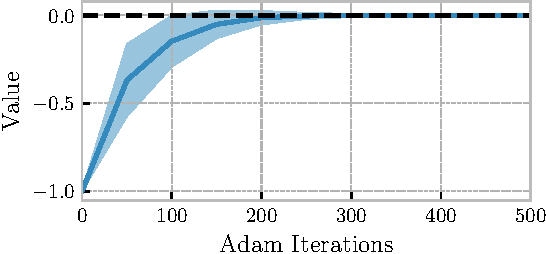
\includegraphics[width=0.49\textwidth]{fig/control-model-free-iter.pdf}
  \hfill
  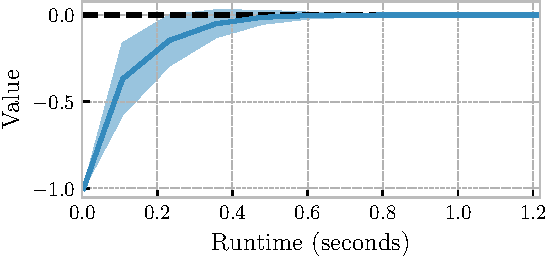
\includegraphics[width=0.49\textwidth]{fig/control-model-free-time.pdf} \\[5mm]
  \cblock{0}{0}{0} Policy $\pi(x)$ --- runtime: 0.65ms
  \caption{
    Runtime comparison between Adam and a learned policy $\pi_\theta$
    to solve \cref{eq:Q-opt} on the humanoid MDP.
    This was evaluated as a batch on an expert trajectory with
    1000 states and was run on an unloaded NVIDIA Quadro GP100 GPU.
    The values are normalized so that $\pi(x)=0$ takes a value of -1 and
    the optimal $\pi^\star$ takes a value of 0.
    The amortized policy is approximately
    1000 times faster than solving the
    problem from scratch.
  }
  \label{fig:model-free-performance}
\end{figure}


This section dives into the training and evaluation code for learning a
deterministic model-free policy $\pi_\theta: \gX\rightarrow\gY$ to amortize a model-free
value estimate $Q$ for controlling the humanoid MDP from
\citet{brockman2016openai}
visualized in \cref{fig:overview}.
This MDP has $|\gX|=45$ states (angular positions and velocities
describing the state of the system)
and $|\gY|=17$ actions (torques to apply to the joints).
A model-free policy $\pi$ maps the state to the optimal actions
that maximize the value on the system.
Given a known action-conditional value estimate $Q(x,u)$,
the optimal policy $\pi^\star$ solves the optimization problem in
\cref{eq:Q-opt} that the learned policy $\pi$ tries to match,
\eg using policy gradient in \cref{eq:dpg-loss}.

The codebase behind \citet{amos2021model} at
\url{https://github.com/facebookresearch/svg}
contains trained model-free policy and value estimates
on the humanoid in addition to model-based components
the next section will use.
The full training code there involves parameterizing
a stochastic policy and estimating many additional
model-based components, but the basic training loop
for amortizing a deterministic policy from the solution
there can be distilled into a form similar to
\cref{lst:vae}.

This section mostly focuses on evaluating the performance
of the trained model-free policy in comparison
to maximizing the model-free value estimate
\cref{eq:Q-opt} from scratch for every state encountered.
An exhaustive evaluation of a solver for \cref{eq:Q-opt}
would need to ensure that the solution is not overly
adapted to a bad part of the $Q$ estimate space ---
because $Q$ is also a neural network susceptible to
adversarial examples, it is very likely that directly
optimizing \cref{eq:Q-opt} may result in a deceptively
good policy when looking at the $Q$ estimate that does not
work well on the real system.
For simplicity, this section ignores these
issues and normalizes the values to $[-1,0]$ where
$-1$ will correspond to the value from taking a zero
action and $0$ will correspond to the value
from taking the expert's action.
(This is valid in this example because the zero
action and expert action never coincide.)

\Cref{fig:model-free-performance} shows that the
amortized policy is approximately 1000 times faster
than solving the problem from scratch.
The $Q$ values presented there are normalized and clamped
so that the expert policy has a value of zero and
the zero action has a value of -1.
This example can be run with
\path{code/evaluate_amortization_speed_function_control.py},
which shares the evaluation code also used for the VAE
in \cref{lst:evaluation}.

\subsection{Control with a model-based value estimate}
\label{sec:impl:model-based}

Extending the results of \cref{sec:impl:model-free},
this section compares the trained humanoid policy
from \url{https://github.com/facebookresearch/svg}
to solving a short-horizon ($H=3$) model-based control
optimization problem defined in \cref{eq:mpc}.
The optimal action sequence solving \cref{eq:mpc}
is $u^\star_{1:H}$ can be approximated by interleaving
a model-free policy $\pi_\theta$ with the dynamics $f$.
While standard model predictive control method are
often ideal for solving for $u^\star_{1:H}$ from scratch,
using Adam as a gradient-based shooting method is
a reasonable baseline in this short-horizon setting.

\Cref{fig:model-based-performance} shows that the
amortized policy is approximately 700 times faster
than solving the problem from scratch.
This model-based setting has the same issues with
the approximation errors in the models and the
model-based value estimate is again
normalized and clamped so that the expert
policy has a value of zero and the zero action has a value of -1.
The source code behind this example is also available in
\path{code/evaluate_amortization_speed_function_control.py}.

\begin{figure}[t]
  \centering
  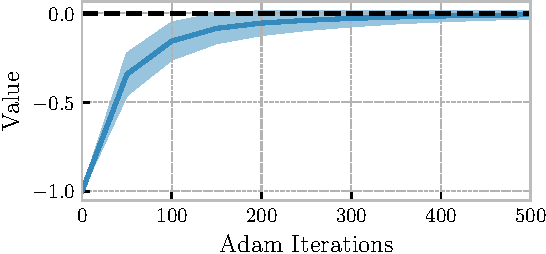
\includegraphics[width=0.49\textwidth]{fig/control-model-based-iter.pdf}
  \hfill
  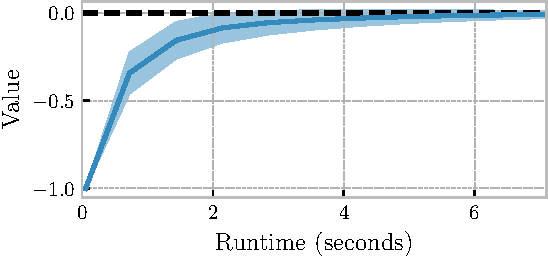
\includegraphics[width=0.49\textwidth]{fig/control-model-based-time.pdf} \\[5mm]
  \cblock{0}{0}{0} Policy $\pi(x)$ --- runtime: 5.8ms
  \caption{Runtime comparison between Adam and a learned policy $\pi_\theta$
    to solve a short-horizon ($H=3$) model-based control
    problem (\cref{eq:mpc}) on the humanoid MDP.
    This was evaluated as a batch on an expert trajectory with
    1000 states and was run on an unloaded NVIDIA Quadro GP100 GPU.
    The amortized policy is approximately
    700 times faster than solving the
    problem from scratch.
  }
  \label{fig:model-based-performance}
\end{figure}

\section{Training an amortization model on a sphere}
\label{sec:impl:sphere}

This section contains a new demonstration that applies
the insights from amortized optimization to learn to solve
optimization problems over spheres of the form
\begin{equation}
  y^\star(x) \in \argmin_{y\in\gS^2} f(y; x),
  \label{eq:sphere-opt-con}
\end{equation}
where $\gS^2$ is the surface of the \emph{unit 2-sphere}
embedded in $\R^3$ as $\gS^2\defeq \{y\in\R^3 \mid \|y\|_2=1\}$
and $x$ is some parameterization of the function
$f: \gS^2\times\gX\rightarrow \R$.
\Cref{eq:sphere-opt-con} is relevant to physical and
geographical settings seeking the extreme values of a
function defined on the Earth or other spaces that can
be approximated with a sphere.
The full source code behind this experiment is available
in \path{code/train-sphere.py}.

\textbf{Amortization objective.}
\Cref{eq:sphere-opt-con} first needs to be transformed
from a constrained optimization problem into an unconstrained
one of the form \cref{eq:opt}.
In this setting, one way of doing this
is by using a projection:
\begin{equation}
  y^\star(x) \in \argmin_{y\in\R^3} f(\pi_{\gS^2}(y); x),
  \label{eq:sphere-opt-proj}
\end{equation}
where $\pi_{\gS^2}: \R^3\rightarrow \gS^2$ is the
Euclidean projection onto $\gS^2$, \ie,
\begin{equation}
  \begin{aligned}
    \pi_{\gS^2}(x)\defeq& \argmin_{y\in\gS^2} \|y-x\|_2 \\
     =& \;x/\|x\|_2.
  \end{aligned}
  \label{eq:pi}
\end{equation}

\textbf{$c$-convex functions on the sphere.}
A synthetic class of optimization problems defined
on the sphere using the $c$-convex functions from
\citet{cohen2021riemannian} can be instantiated with:
\begin{equation}
  f(y; x) = {\textstyle \min_{\gamma}} \left\{\frac{1}{2} d(x,z_i)+\alpha_i\right\}_{i=1}^m
  \label{eq:rcpm}
\end{equation}
where $m$ components define the context
$x=\{z_i\} \cup \{\alpha_i\}$
with $z_i\in\gS^2$ and $\alpha_i\in\R$,
$d(x,y)\defeq \arccos(x^\top y)$ is the
Riemannian distance on the sphere in the
ambient Euclidean space, and
$\min_\gamma(a_1,\ldots,a_m)\defeq -\gamma\log\sum_{i=1}^m\exp(-a_i/\gamma)$
is a soft minimization operator
as proposed in \citet{cuturi2017soft}.
The context distribution $p(x)$ is sampled
with $z_i\sim \gU(\gS^2)$, \ie uniformly from the sphere,
and $\alpha_i\sim\gN(0,\beta)$
with variance $\beta\in\R_+$.

\textbf{Amortization model.}
The model $\hat y_\theta: \gX\rightarrow\R$
is a fully-connected MLP.
The predictions to \cref{eq:sphere-opt-con}
on the sphere can again be obtained by composing
the output with the projection
$\pi_{\gS^2}\circ \hat y_\theta$.

\textbf{Optimizing the gradient-based loss.}
Finally, it is reasonable to optimize the
gradient-based loss $\gL_{\rm obj}$ because
the objective and model are tractable and
easily differentiable.
\Cref{fig:sphere} shows the model's predictions
starting with the untrained model and finishing
with the trained model, showing that this setup
indeed enables us to predict the solutions to
\cref{eq:sphere-opt-con} with a single neural network
$\hat y_\theta(x)$ trained with the gradient-based loss.

\textbf{Summary.}
$\gA_{\rm sphere}\defeq (f\circ \pi_{\gS^2}, \R^3, \gX, p(x), \hat y_\theta, \gL_{\rm obj})$

\begin{figure}
  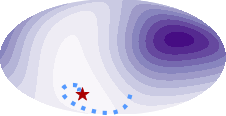
\includegraphics[width=0.25\textwidth]{fig/sphere/0.png}
  \hspace{-2.7mm}
  
\includegraphics[width=0.25\textwidth]{fig/sphere/1.png}
  \hspace{-2.7mm}
  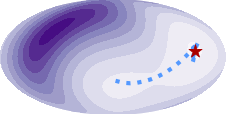
\includegraphics[width=0.25\textwidth]{fig/sphere/2.png}
  \hspace{-2.7mm}
  
\includegraphics[width=0.25\textwidth]{fig/sphere/3.png} \\[-.8mm]
  
\includegraphics[width=0.25\textwidth]{fig/sphere/4.png}
  \hspace{-2.7mm}
  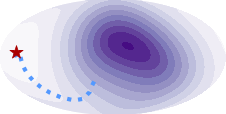
\includegraphics[width=0.25\textwidth]{fig/sphere/5.png}
  \hspace{-2.7mm}
  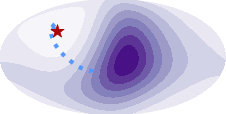
\includegraphics[width=0.25\textwidth]{fig/sphere/6.png}
  \hspace{-2.7mm}
  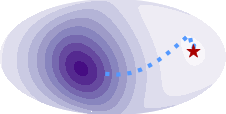
\includegraphics[width=0.25\textwidth]{fig/sphere/7.png} \\[-6mm]
  \begin{center}
    \cblock{73}{19}{134} $f(y; x)$ contours \;
    \cblock{170}{0}{0} Optimal $y^\star(x)$ \;
    \cblock{84}{153}{255} Predictions $\hat y_\theta(x)$ throughout training
  \end{center}
  \vspace{-3mm}
  \caption{Visualization of the predictions of an amortized
    optimization model predicting the solutions
    to optimization problems on the sphere.}
  \label{fig:sphere}
\end{figure}

\section{Other useful software packages}
\label{sec:impl:software}

Implementing semi-amortized models are usually more challenging
than fully-amortized models. Learning an optimization-based
model that internally solves an optimization problem is
not as widespread as learning a feedforward neural network.
While most autodiff packages provide standalone features to implement
unrolled gradient-based optimization, the following specialized
packages provide crucial features that further enable the
exploration of semi-amortized models:
\begin{itemize}
\item \href{https://github.com/cvxgrp/cvxpylayers}{cvxpylayers}
  \citep{agrawal2019differentiable}
  allows an optimization problem to be expressed in the
  high-level language \verb!CVXPY! \citep{diamond2016cvxpy}
  and exported to PyTorch, JAX, and TensorFlow
  as a differentiable optimization layers.
\item \href{https://github.com/google/jaxopt}{jaxopt}
  \citep{blondel2021efficient}
  is a differentiable optimization library for JAX
  and implements many optimization settings and fixed-point
  computations along with their implicit derivatives.
\item \href{https://github.com/facebookresearch/higher}{higher}
  \citep{grefenstette2019generalized}
  is a PyTorch library that adds differentiable higher-order
  optimization support with
  1) monkey-patched functional \verb!torch.nn! modules,
  and 2) differentiable versions of \verb!torch.optim!
  optimizers such as Adam and SGD.
  This enables arbitrary torch modules and optimizers
  to be unrolled and used as a semi-amortized model.
\item \href{https://github.com/metaopt/TorchOpt}{TorchOpt}
  provides a functional and differentiable optimizer in PyTorch
  and has higher performance than \verb!higher! in some cases.
\item \href{https://github.com/pytorch/functorch}{functorch}
  \citep{functorch2021} is a PyTorch library providing
  composable function transforms for batching and
  derivative operations, and for creating functional
  versions of PyTorch modules that can be used in
  optimization algorithms.
  All of these operations may arise in the implementation
  of an amortized optimization method and can become computational
  bottlenecks if not efficiently implemented.
\item \href{https://github.com/jump-dev/DiffOpt.jl}{DiffOpt.jl}
  provides differentiable optimization in Julia's JuMP
  \citep{DunningHuchetteLubin2017}.
\item \href{https://github.com/tristandeleu/pytorch-meta}{Torchmeta}
  \citep{deleu2019torchmeta} and
  \href{http://learn2learn.net}{learn2learn}
  \citep{arnold2020learn2learn}
  are PyTorch libraries and collection of meta-learning
  algorithms that also focus on making data-loading
  and task definitions easy.
\item \href{https://github.com/prolearner/hypertorch}{hypertorch}
  \citep{grazzi2020iteration}
  is a PyTorch package for computing hypergradients with a
  large focus on providing computationally efficient approximations
  to them.
\end{itemize}

%%% Local Variables:
%%% coding: utf-8
%%% mode: latex
%%% TeX-master: "../amor.tex"
%%% LaTeX-biblatex-use-Biber: True
%%% End: